\graphicspath{{./chapitres/chapitre3/figures/}}
\chapter{Sprint Zéro : Initiation au projet }
\minitoc
\newpage
\section*{Introduction}

Avant de commencer le premier sprint, on a un sprint zéro dédié à préparer ce qui est nécessaire au lancement des sprints dans de bonnes conditions.\\
Le sprint est le coeur de Scrum. Il s'agit d'un bloc de temps durant lequel un incrément du produit sera réalisé. Tous les sprints d'une release ont une durée constante et ne se chevauchent jamais, c'est-à-dire qu'un sprint ne peut pas démarrer tant que le précédent n'est pas encore terminé. 




\section{Sprint Backlog}
\subsection{Les histoires à réaliser}
Avant de se lancer dans un sprint, l'équipe Scrum doit obligatoirement définir le but de ce dernier qui doit être un tableau descriptif qui précise la charge de travail pour chaque tâche. Le tableau \ref{tab:sprint_0_backlog} décrit les histoires à réaliser durant ce sprint.
\newpage
\begin{table}[!ht]
    \center
\begin{tabular}{|l|l|c|}
\hline
{\textbf{Feature}} & {\textbf{User Story}} & {\textbf{Story point}}\\
\hline
\multirow{2}{3cm}{\textbf{ Une formation Spring Boot}} &  R\&D Spring Boot & 3 \\
\cline{2-3}
& R\&D Spring REST, Spring Data et & 5\\&la bibliothèque Lombok & \\
\hline
\multirow{2}{3cm}{\textbf{ Une formation Python et Flask}} & R\&D Python   & 3 \\
\cline{2-3}
& R\&D Flask et Flask-MongoEngine  & 5 \\
\cline{2-3}
&  R\&D algorithme data mining & 3 \\
\hline
\multirow{2}{4cm}{\textbf{Une formation Angular 7}} & Une Recherche sur sa structure   &  3\\
\cline{2-3}
& Une recherche sur la liaison entre l’Angular & 3 \\
&et Spring ou python &\\

\hline
\multirow{2}{4cm}{\textbf{Une formation MongoDB }} & Une formation sur la bases de données NoSql  & 3\\
& MongoDB &\\
\hline
\multirow{2}{4cm}{\textbf{Mise en place de l’environnement de travail}} 
&- Installation et téléchargement  &3\\ 
&  des outils de travail &  \\
& - Création des comptes gitlab et Jira & \\
\hline
\end{tabular}
\caption{Liste des tâches du Sprint zéro}
\label{tab:sprint_0_backlog}
\end{table}

\subsection{L'objectif du sprint}
L'objectif de ce sprint est de mettre en place des fondations techniques en début de projet. En effet, nous avons étudié les avantages de la base de données MongoDB . Nous avons également effectué une recherche sur GitLab et enfin mis en place l'environnement de travail nécessaire.
 \paragraph{Avantages de MongoDB}



\subsection{Environnement logiciel}
Pour accomplir notre mission, nous nous sommes servis de plusieurs ressources logicielles.
\subsubsection*{WebStorm}
C'est un IDE pour les langages Web (HTML, CSS et JavaScript), d\'evelopp\'e par l'entreprise JetBrains et bas\'e sur la plateforme IntelliJ IDEA.
\begin{figure}[!ht]\centering

\includegraphics[width=0.2\textwidth]{chapitres/chapitrex/figures/webstorm_logo.png}
\caption{webStorm logo}
\label{fig:webstorm_logo}
\end{figure}

\subsubsection*{IntelliJ IDEA}
IntelliJ IDEA est un IDE Java commercial d\'evelopp\'e par JetBrains. Il est fr\'equemment appel\'e par le simple nom de : "IntelliJ", "IDEA" ou "IDJ".
\begin{figure}[!ht]\centering

\includegraphics[width=0.2\textwidth]{chapitres/chapitre3/figures/intellij-idea_logo.png}
\caption{intellijIdea log}
\label{fig:intellij-idea_log}
\end{figure}
\subsubsection*{PyCharm }
PyCharm  st un environnement de développement intégré utilisé pour programmer en Python,  d\'evelopp\'e par l'entreprise JetBrains .
\begin{figure}[!ht]\centering

\includegraphics[width=0.2\textwidth]{chapitres/chapitrex/figures/pycharme.png}
\caption{Pycharm logo}
\label{fig:pycharme}
\end{figure}
\subsubsection*{JIRA Software}
JIRA est un outil de gestion de projet Agile qui prend en charge toute m\'ethodologie Agile telle que Scrum. Il permet \`a une \'equipe de d\'eveloppement, de planifier, de suivre et de livrer un bon logiciel de qualit\'e sup\'erieure rapidement. Il permet aussi de g\'en\'erer des rapports pour am\'eliorer les performances de l'\'equipe.
\subsubsection*{GitLab}
Nous avons travaill\'e tout le long de notre projet sur Gitlab. Celui-ci est un gestionnaire de d\'ep\^ots Git licenci\'e open source et bas\'e sur le Web offrant des fonctionnalit\'es de partage, de suivi et de contr\^ole de versions des projets de d\'eveloppements.

\subsubsection*{Postman}
Postman Permet aux \'equipes de toutes tailles de collaborer de mani\`ere transparente en temps r\'eel sur des espaces de travail et des collections partag\'ees. Les espaces de travail des \'equipes. Postman permettent aux \'equipes de rester organis\'ees et de conserver une source de v\'erit\'e unique tout au long du cycle de d\'eveloppement de l'API \cite{Postman}.
\begin{figure}[!ht]\centering

\includegraphics[width=0.4\textwidth]{chapitres/chapitrex/figures/postman.png}
\caption{Postman logo}
\label{fig:postman}
\end{figure}
\subsubsection*{Apache Tomcat 9}
Tomcat est un serveur d'applications Java. Nous avons déjà présenté ce qu'est une application web. Elle permet de générer une réponse HTML à une requête après avoir effectué un certain nombre d'opérations (connexion à une base de données, à un annuaire LDAP...). Pour le client (un navigateur web en général), il n'y a pas de différence avec une page web statique : il reçoit toujours du HTML, seul langage qu'il comprend. Seule la manière dont la réponse est formée côté serveur change.
\begin{figure}[!ht]\centering

\includegraphics[width=0.4\textwidth]{chapitres/chapitre3/figures/apachtomcat.png}
\caption{Apache Tomcat logo}
\label{fig:apachtomcat}
\end{figure}
\subsubsection*{Robo 3T}
Anciennement Robomongo, Robo 3T est une interface graphique l\'eg\`ere gratuite pour les amateurs de MongoDB.
\begin{figure}[!ht]\centering

\includegraphics[width=0.2\textwidth]{chapitres/chapitrex/figures/robot3t.png}
\caption{Robo 3T logo}
\label{fig:robot3t}
\end{figure}

\subsection{Argumentation des choix techniques}
Dans cette partie, nous d\'etaillons les choix technologiques qui ont \'et\'e pris en compte afin de r\'ealiser la solution. Notre application se base en effet principalement sur l'\'ecosyst\`eme Spring qui rend possible d'aboutir \`a des applications complexes et passantes \`a l'\'echelle en un temps court.
\subsubsection*{Spring}
C'est un  framework libre pour le d\'eveloppement d'applications, principalement d'entreprises.

Il fournit de nombreuses fonctionnalit\'es qui peuvent \^etre configur\'ees ou utilis\'ees de plusieurs mani\`eres : ceci laisse le choix au d\'eveloppeur d'utiliser la solution qui lui convient le mieux et/ou qui r\'epond aux besoins.

Spring est ainsi un des frameworks les plus r\'epandus dans le monde Java. Sa popularit\'e a grandi au profit de la complexit\'e de Java EE notamment pour ses versions ant\'erieures \`a la version 5 mais aussi gr\^ace \`a la qualit\'e et la richesse des fonctionnalit\'es qu'il propose : 
\begin{itemize}
\item Son coeur reposant sur un conteneur de type IoC assure la gestion du cycle de vie des beans et l'injection des d\'ependances.
\item L'utilisation de l'AOP. 
\item Une grande flexibilit\'e dans les fonctionnalit\'es et les projets utilis\'es dans une application.
\end{itemize}
Spring offre tout un \'ecosyst\`eme qui g\`ere plusieurs couches afin de permettre une s\'eparation entre ces couches mais avec une solide int\'egrit\'e \cite{spr}.
\newpage
\begin{figure}[!ht]\centering
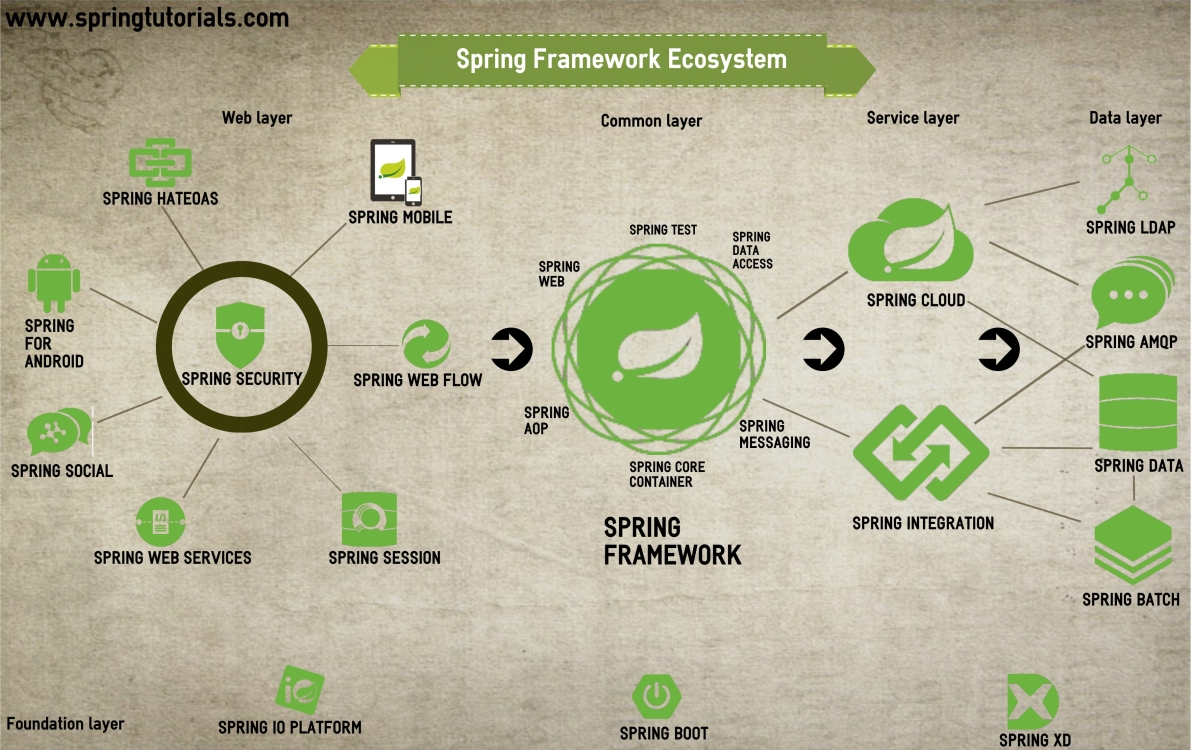
\includegraphics[width=0.8\textwidth]{chapitres/chapitrex/figures/spring-ecosystem.jpg}
\caption{Spring-ecosystem}
\label{fig:spring-ecosystem}
\end{figure}
\subsubsection*{Spring Boot}
Spring Boot est un nouveau framework cr\'e\'e par Pivotal pour simplifier le d\'eveloppement de nouvelles applications Spring en proposant une approche dogmatique de la configuration. Cette configuration automatique offerte par Spring boot permet d'\'eviter la red\'efinition de la m\^eme configuration dans plusieurs endroits du code.

Les applications \'ecrites \`a l'aide de Boot restent concises tout en offrant beaucoup de fonctionnalit\'es \cite{SpringBoot}.
\begin{figure}[!ht]\centering
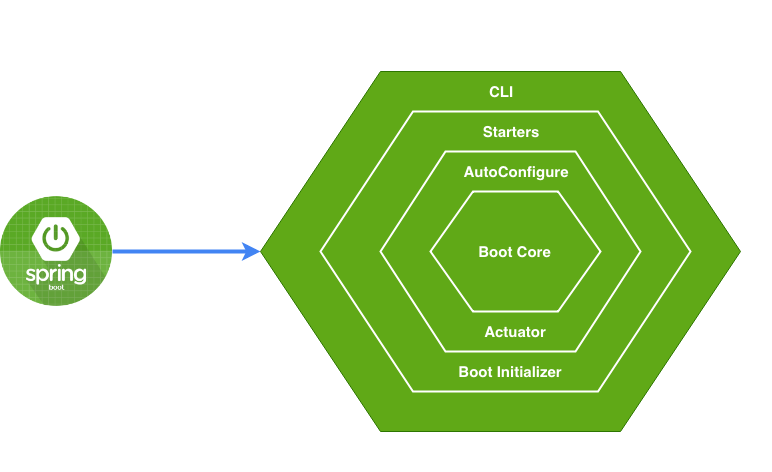
\includegraphics[width=0.8\textwidth]{chapitres/chapitrex/figures/Spring-Boot-Modules.png}
\caption{Spring Boot Modules}
\label{fig:Spring-Boot-Modules}
\end{figure}
\subsubsection*{Spring Data}
Spring Data est une couche d'abstraction commune \`a de multiples sources de donn\'ees. Cette couche permet de r\'epondre aux besoins de manipulation des donn\'ees d'une mani\`ere plus simple. Elle offre un ensemble de repositories(r\'epertoires) pr\^et \`a l'utilisation pour l'acc\`es aux donn\'ees car ils construisent une couche d’abstraction qui r\'eduit le code n\'ecessaire pour impl\'ementer l'acc\`es aux donn\'ees pour des diverses types d'outils de stockage. 

Dans notre cas, nous allons travailler avec MongoDB Repository qui nous offre un acc\`es simple et rapide \`a nos donn\'ees stock\'ees et nous facilite ainsi la manipulation de celles-ci sans avoir besoin \`a impl\'ementer des requ\^etes. La figure \ref{fig:architecture_springdata}  
\cite{nosql} illustre l'architecture de Spring Data pour son int\'egration avec MongoDB.
\begin{figure}[!ht]\centering
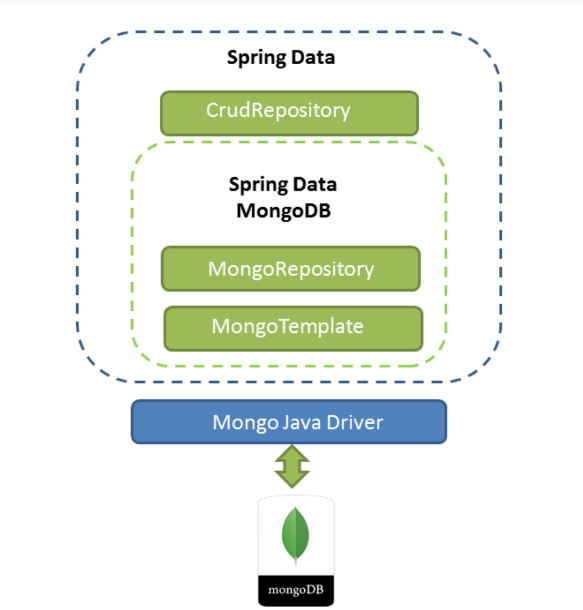
\includegraphics[width=0.8\textwidth]{chapitres/chapitrex/figures/SpringData.png}
\caption{Architecture de Spring Data avec MongoDB}
\label{fig:architecture_springdata}
\end{figure}

\subsubsection*{Spring REST}
REST est un style architectural pour la conception de syst\`emes distribu\'es. Il n'est pas une norme, mais un ensemble de contraintes, ayant une relation client/serveur et une interface uniforme. REST n'est pas strictement li\'ee à HTTP, mais il est le plus souvent associ\'e. Nous \'enum\'erons les principes de REST qui nous facilitent la vie :
\begin{itemize}
\item Les ressources expos\'ees sont faciles \`a comprendre gr\^ace \`a la structure des adresses URIs. 
\item La repr\'esentations de transfert JSON ou XML pour repr\'esenter des objets de donn\'ees et leurs attributs. 
\item Les messages utilisent des m\'ethodes HTTP de mani\`ere explicite (par exemple GET, POST, PUT et DELETE). 
\item Les interactions "stateless" ne stockent pas de contexte de client sur le serveur entre les requ\^etes.

\end{itemize}
\begin{figure}[!ht]\centering
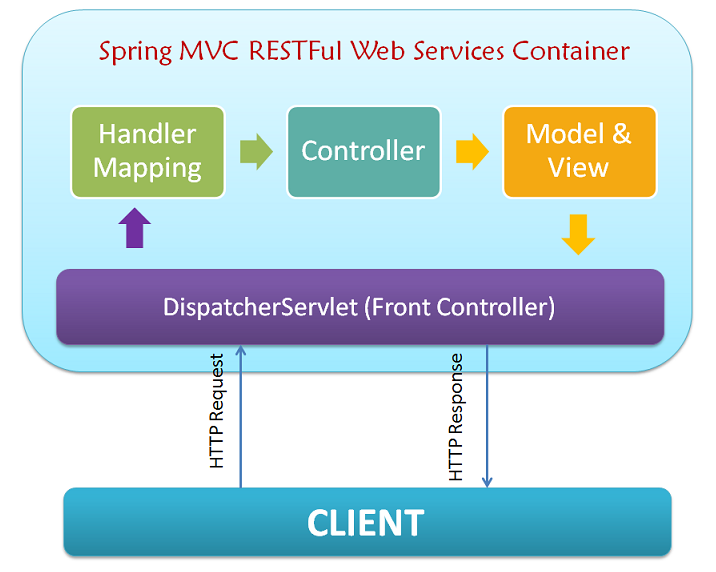
\includegraphics[width=0.8\textwidth]{chapitres/chapitrex/figures/springRest.png}
\caption{Spring Rest }
\label{fig:springRest}
\end{figure}
\subsubsection*{Python}
Python est un langage de programmation interprété, orienté objet et de haut niveau avec une sémantique dynamique. Ses structures de données intégrées de haut niveau, combinées à un typage dynamique et à une liaison dynamique, le rendent très attrayant pour le développement rapide d'applications, ainsi que pour son utilisation en tant que langage de script ou de collage pour connecter des composants existants. La syntaxe simple et facile à apprendre de Python met l'accent sur la lisibilité et réduit donc le coût de la maintenance du programme. Python prend en charge les modules et les packages, ce qui encourage la modularité du programme et la réutilisation du code. L'interpréteur Python et la vaste bibliothèque standard sont disponibles gratuitement sous forme binaire ou source pour toutes les principales plates-formes et peuvent être distribués librement.
\begin{figure}[!ht]\centering

\includegraphics[width=0.4\textwidth]{chapitres/chapitrex/figures/python.png}
\caption{Python logo }
\label{fig:python}
\end{figure}
\subsubsection*{Flask}
Flask est un micro-framework web écrit en Python. Il s’agit d’un microframework car il ne nécessite ni outils ni bibliothèques particuliers. ... Cependant, Flask prend en charge des extensions pouvant ajouter des fonctionnalités d'application comme si elles étaient implémentées dans Flask même.
\begin{figure}[!ht]\centering

\includegraphics[width=0.4\textwidth]{chapitres/chapitrex/figures/flask.png}
\caption{Flask logo }
\label{fig:flask}
\end{figure}
\subsubsection*{Frameworks Web}
Pour la partie purement Web de notre application, nous avons choisi les frameworks web suivants :
\paragraph{Angular 7}
C'est un framework Javascript libre open source d\'evelopp\'e par Google. Il est cr\'e\'e sur l'extension du langage HTML en ajoutant de nouvelles balises et attributs. Le code HTML pr\'esente  alors la partie vue du patron d'architecture MVC (mod\`ele vue controleur), les "scopes" jouent le r\^ole de mod\`eles qui sont manipul\'es par le contrôleur pour d\'efinir les actions avec du javascript imp\'eratif. Angular est une r\'e\'ecriture compl\`ete de AngularJS, cadriciel construit par la m\^eme \'equipe.
\begin{figure}[!ht]\centering

\includegraphics[width=0.4\textwidth]{chapitres/chapitrex/figures/angular.png}
\caption{Angular logo }
\label{fig:angular}
\end{figure}




\section*{Conclusion}
Dans ce chapitre, nous avons pr\'esent\'e dans un premier release la gestion des donn\'ees m\'etiers repr\'esent\'ee par quatre sprints \`a savoir : la mise en place des fondations du projet dans le sprint z\'ero, la gestion des utilisateurs dans le premier sprint, la gestion des groupes dans le deuxi\`eme sprint et le troisi\`eme sprint s'articule sur la gestion des r\^oles.

Dans le chapitre suivant, nous pr\'esentons la gestion des donn\'ees de configuration dans une deuxi\'eme release qui est divis\'ee en deux sprints : le premier sprint est repr\'esent\'e par la gestion de l'authentification et le deuxi\`eme sprint est repr\'esent\'e par les tableaux de bord des statistiques.